%% Dexter Barrows, 2016
%% dbarrows.github.io

\section{Data Setup}

	This section will focus on taking the stochastic SIR model from the previous section, truncating the synthetic data output from realizations of that model, and seeing how well IF2 and HMCMC can reconstruct out-of-sample forecasts.

	An example of a simulated system with truncated data can be seen in Figure [\ref{dataplot}] below.

	\begin{figure}[H]
        \centering
        \captionsetup{width=.8\linewidth}
        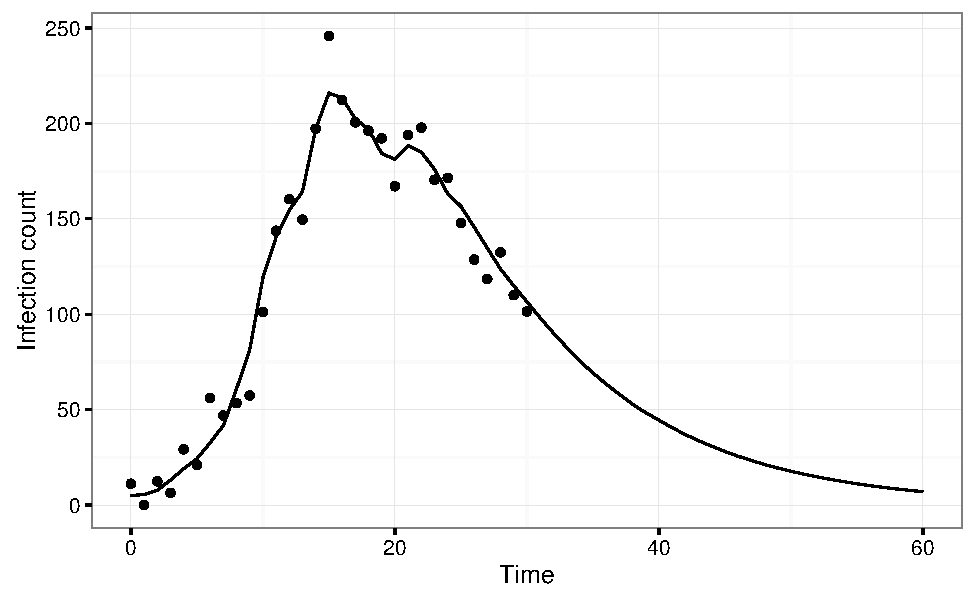
\includegraphics[width=0.8\textwidth]{./images/dataplot.pdf}
        \caption{Infection count data truncated at $T = 30$. The solid line shows the true underlying system states, and the dots show those states with added observation noise. Parameters used were $R_0 = 3.0$, $r = 0.1$, $\eta = .05$, $\sigma_{proc} = 0.5$, and additive observation noise was drawn from $\mathcal{N}(0,10)$.}
        \label{dataplot}
    \end{figure}

	In essence we want to be able to give either IF2 of HMCMC only the data points and have it reconstruct the entirety of the true system states.
    

\section{IF2}

	For IF2, we will take advantage of the fact that the particle filter will produce state estimates for every datum in the time series given to it, as well as producing parameter maximum likelihood point estimates. Both of these sources of information will be used to produce forecasts by parametric bootstrapping using the final parameter estimates from the particle swarm after the last IF2 pass, then using the newly generated parameter sets along with the system state point estimates from the first fitting to simulate the systems forward into he future.

	We will truncate the data at half the original time series length (to $T = 30$), and fit the model as previously described.

	First, we can see the state estimates for each time point produced by the last IF2 pass in Figure [\ref{if2fit}] below.

	\begin{figure}[H]
        \centering
        \captionsetup{width=.8\linewidth}
        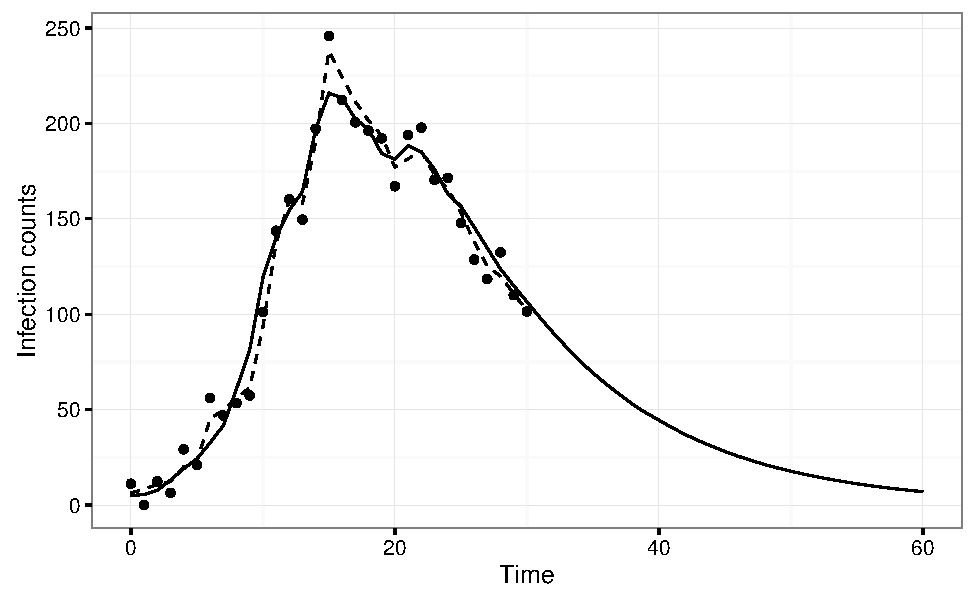
\includegraphics[width=0.8\textwidth]{./images/if2fit.pdf}
        \caption{Infection count data truncated at $T = 30$ from Figure [\ref{dataplot}] above. The dashed line shows IF2's attempt to reconstruct the true underlying state from the observed data points.}
        \label{if2fit}
    \end{figure}

    Recall that IF2 is not trying to generate parameter estimation densities, but rather produce a point estimate. Since we wish to determine the approximate distribution of each of the parameters in addition to the point estimate, we must turn to another method, parametric bootstrapping.


\subsection{Parametric Bootstrapping}

	The goal of the parametric bootstrap is use an initial density sample $\theta^*$ to generate further samples $\theta_1, \theta_2, ..., \theta_M$. It works by using $\theta$ to generate artificial data sets $D_1, D_2, ..., D_M$ to which we can refit our model of interest and generate new parameter sets.

	\textit{[I'm still trying to dig up a good paper that talks about applicability to dynamical systems, there will be a paragraph here about it.]}

	An algorithm for parametric bootstrapping using IF2 and our stochastic SIR model is shown in Algorithm [\ref{paraboot}].

	\begin{algorithm}[H]

        \BlankLine

        \SetKwInOut{Input}{Input}
        \SetKwInOut{Output}{Output}
        \DontPrintSemicolon

        \Input{Forward simulator $S(\theta)$, data set D}

        \BlankLine

        \tcc{Initial fit}
        $\theta^* \gets IF2(D)$

        \BlankLine

        \tcc{Generate artificial data sets}
        \For{$i = 1:M$}{
	        $D_i \gets S(\theta^*)$
        }

        \BlankLine

        \tcc{Fit to new data sets}
        \For{$i = 1:M$}{
	        $\theta_i \gets IF2(D_i)$
        }

        \BlankLine

        \Output{Distribution samples $\theta_1, \theta_2, ..., \theta_M$}

        \caption{Parametric Bootstrap}\label{paraboot}

    \end{algorithm}
	

\subsection{IF2 Forecasts}

	Using the parameter sets $\theta_1, \theta_2, ..., \theta_M$ and the point estimate of the state provided by the initial IF2 fit, we can use a normal bootstrap to produce estimates of the future state. A plot showing a projection of the data from the previous plots can be seen in Figure [\ref{if2combined}].

	\begin{figure}[H]
        \centering
        \captionsetup{width=.8\linewidth}
        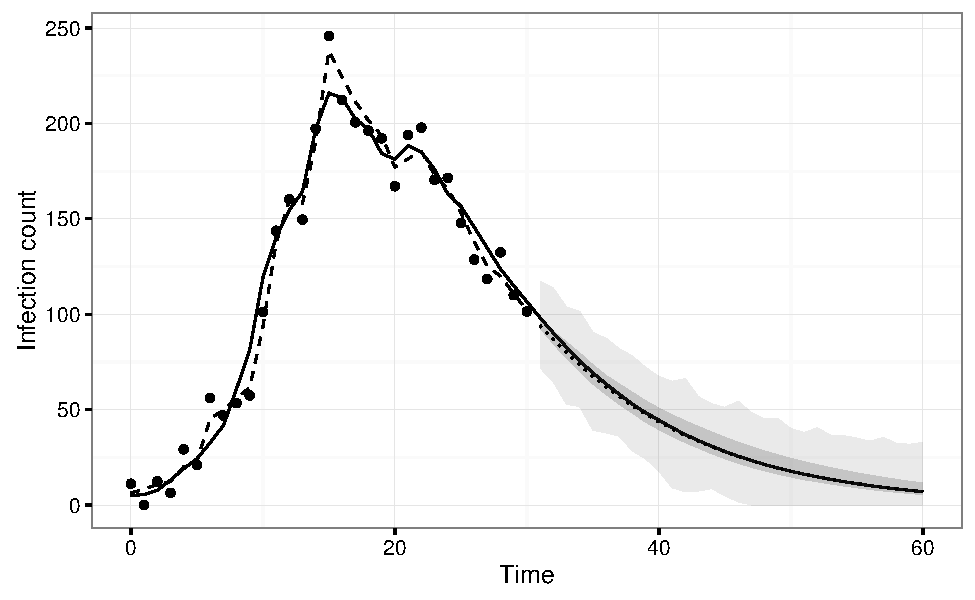
\includegraphics[width=0.8\textwidth]{./images/if2combined.pdf}
        \caption{Forecast produced by the IF2 / parametric bootstrapping framework. The dotted line shows the mean estimate of the forecasts, the dark grey ribbon shows the centre 95th quantile of the true state estimates, and the lighter grey ribbon shows the centre 95th quantile of the true state estimates with added observation noise drawn from $\mathcal{N}(0,\sigma)$.}
        \label{if2combined}
    \end{figure}

    We can define a metric to gauge forecast effectiveness by calculating the SSE and dividing that value by the number of values predicted to get the average squared error per point. For the data in Figure [\ref{if2combined}] the value was $\overline{SSE} = 1.67$.
    

\section{HMCMC}

	For HMCMC we can use a simpler bootstrapping approach. We do not get state estimates directly from the RStan fitting due to the way we implemented the model, but we can construct them using the process noise latent variables. Once we've done this we can forward simulate the system from the state estimate into the future.

	As before we fit the stochastic SIR model to the partial data, but now perform bootstrapping as described above, and obtain the plot in Figure [\ref{hmcforecast}].

	\begin{figure}[H]
        \centering
        \captionsetup{width=.8\linewidth}
        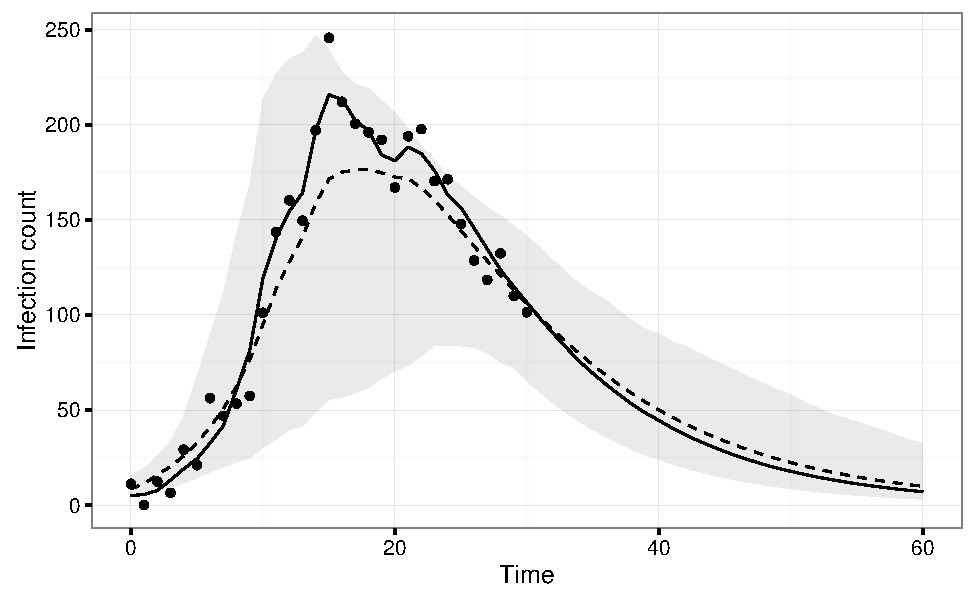
\includegraphics[width=0.8\textwidth]{./images/hmcforecast.pdf}
        \caption{Forecast produced by the HMCMC / bootstrapping framework with $M = 200$ trajectories. The dotted line shows the mean estimate of the forecasts, and the grey ribbon shows the centre 95th quantile.}
        \label{hmcforecast}
    \end{figure}

    And as before we can evaluate the averaged SSE of the forecast for the data shown, giving $\overline{SSE} = 20.27$.


\section{Truncation vs. Error}

	Of course the above mini-comparison only shows one truncation value for one trajectory. Really, we need to know how each method performs on average given different trajectories and truncation amounts. In effect we wish to ``starve'' each method of data and see how poor the estimates become with each successive data point loss.

	Using each method, we can fit the stochastic SIR model to successively smaller time series to see the effect of truncation on forecast averaged SSE. This was performed with 10 new trajectories drawn for each of the desired lengths. The results are shown in Figure [\ref{truncation}].

	\begin{figure}[H]
        \centering
        \captionsetup{width=.8\linewidth}
        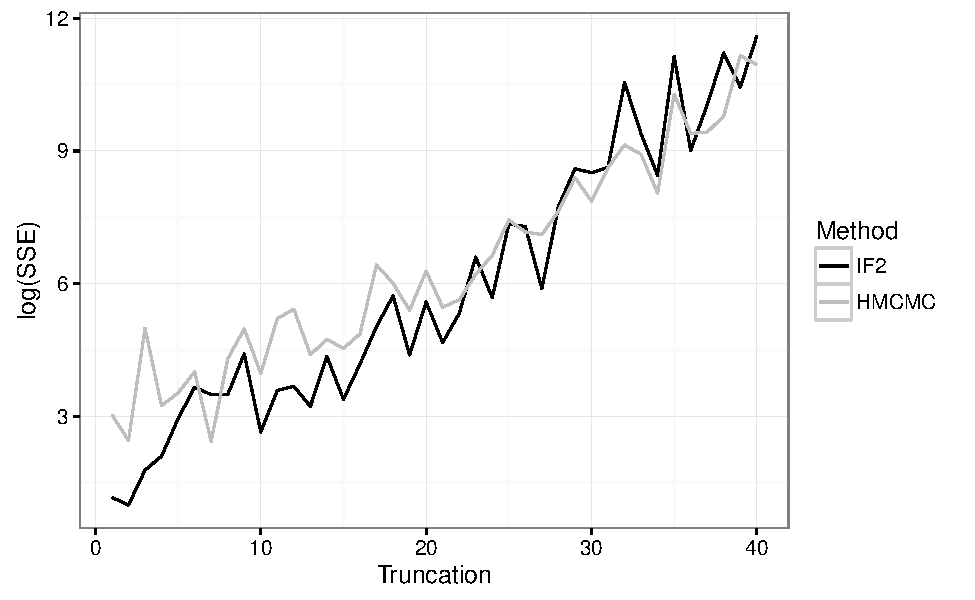
\includegraphics[width=0.8\textwidth]{./images/truncation.pdf}
        \caption{Error growth as a function of data truncation amount. Both methods used 200 bootstrap trajectories. Note that the y-axis shows the natural log of the averaged SSE, not the total SSE.}
        \label{truncation}
    \end{figure}

    IF2 and HMCMC perform very closely, with IF2 maintaining a small advantage up to a truncation of about 25-30 data points.

    Since the parametric bootstrapping approach used by IF2 requires a significant number of additional fits, its computational cost is significantly higher than the simpler bootstrapping approach used by the HMCMC framework, about 35.5x as expensive. However the now much longer running time can somewhat alleviated by parallelizing the parametric bootstrapping process; as each of the parametric bootstrap fittings in entirely independent, this can be done without a great deal of additional effort. The code used here has this capability, but it was not utilised in the comparison so as to accurately represent total computational cost, not potential running time.